\section{TP over dense temporal domains is an undecidable problem}\label{sec:undecidability}

In this section, we
start by settling an important negative result, namely, we
show that the TP problem, in its full generality, is undecidable over dense temporal domains, even when a single state variable is involved.
Undecidability is proved via a reduction from the halting problem for \emph{Minsky $2$-counter machines}~\cite{Minsky67}. The proof somehow resembles the one for the satisfiability problem of Metric Temporal Logic (which will be formally introduced later, in Section~\ref{sec:DecisionProcedures}) with both past and future temporal modalities, interpreted on dense time~\cite{AlurH93}.

As a preliminary step, we give a short account of Minsky 2-counter machines. A Minsky 2-counter machine (or just \emph{counter machine} for short) is a tuple $M = \tpl{\Instruct,\ell_\init,\ell_\halt}$ consisting of a finite set $\Instruct$ of labeled instructions $\ell: \imath$, where $\ell$ is a label  and $\imath$ is an instruction for either
\begin{itemize}
  \item \emph{increment} of counter $h$: $c_h:= c_h+1$; \texttt{goto} $\ell_r$, or
  \item  \emph{decrement} of counter $h$: \texttt{if} $c_h\!>\!0$ \texttt{then} $c_h:= c_h-1$; \texttt{goto} $\ell_s$ \texttt{else goto} $\ell_t$,
\end{itemize}
where $h \in \{1, 2\}$,  $\ell_s\neq \ell_t$, and $\ell_r$ (respectively, $\ell_s, \ell_t$) is either a label of an instruction in $\Instruct$ or the halting label $\ell_\halt$. Moreover, $\ell_\init\in\Instruct$ is the label of a designated (\lq\lq initial\rq\rq) instruction.

An \emph{$M$-configuration} is a triple of the form $C=(\ell, n_1, n_2)$, where $\ell$ is the label of an instruction (intuitively, which is the one to be executed next), and $n_1,n_2\in\Nat$ are the current values of the two counters $c_1$ and $c_2$, respectively. 

$M$ induces a transition relation, denoted by $\stackrel{M}{\longrightarrow}$, over pairs of $M$-configurations: 
\begin{itemize}
    \item for an instruction with label $\ell$ incrementing $c_1$, we have $(\ell, n_1, n_2)\stackrel{M}{\longrightarrow} (\ell_r, n_1+1, n_2)$, and
    \item for an instruction decrementing $c_1$, we have $(\ell, n_1, n_2)\stackrel{M}{\longrightarrow} (\ell_s, n_1-1, n_2)$ if $n_1>0$, and $(\ell, 0, n_2)\stackrel{M}{\longrightarrow} (\ell_t, 0, n_2)$ otherwise. 
\end{itemize}
The analogous for instructions changing the value of $c_2$.

An \emph{$M$-computation} is a \emph{finite} sequence $C_1,\ldots ,C_k$ of $M$-configurations such that $C_i \stackrel{M}{\longrightarrow} C_{i+1}$ for all $1\leq i<k$.
%
$M$ \emph{halts} if there exists an $M$-computation starting at $(\ell_\init, 0, 0)$ and leading to 
$(\ell_{\halt}, n_1, n_2)$, for some $n_1,n_2\in\Nat$. 
Given a counter machine $M$,
the \emph{halting problem for $M$} is to decide whether $M$ halts, and it was proved to be \emph{undecidable} by Minsky~\cite{Minsky67}.

The rest of the section is devoted to showing the following result.
\begin{theorem}\label{theorem:undecidability}
The TP problem over dense temporal domains is undecidable (even when a single state variable is involved).
\end{theorem}
\begin{proof}
We prove the thesis by a reduction from the halting problem for Minsky $2$-counter machines. 
%
Let us introduce the following notational conventions:
\begin{itemize}
  \item for increment instructions $\ell : c_h:= c_h+1$; \texttt{goto} $\ell_r$, we define $c(\ell)= c_h$ and $\Succ(\ell)= \ell_r$;
  \item  for decrement instructions $\ell:$ \texttt{if} $c_h>0$ \texttt{then} $c_h:= c_h-1$; \texttt{goto}  $\ell_r$ \texttt{else goto} $\ell_s$,
  we define $c(\ell)= c_h$, $\dec(\ell)= \ell_r$, and $\zero(\ell)= \ell_s$.
\end{itemize}
Moreover, let $\InstructLab$ be the set of instruction labels, including $\ell_\halt$, and let
$\Inc$ (resp., $\Dec$) be the set of labels for increment (resp., decrement) instructions.
%
We consider a counter machine $M = \tpl{\Instruct,\ell_\init,\ell_\halt}$ assuming without loss of generality that
no instruction of $M$ leads to $\ell_\init$, and that $\ell_\init$ is the label of an increment instruction.
To prove the thesis, we build in polynomial time a state variable $x_M=(V,T,D)$ and a finite set $R_M$ of synchronization rules
over $x_M$ such that $M$ halts if and only if there is a timeline for $x_M$ which satisfies all the rules in $R_M$, that is, a plan for $P=(\{x_M\},R_M)$.
%The thesis immediately follows. 

\paragraph*{Encoding of $M$-computations.}

First, we define a suitable encoding of a computation of $M$ as a timeline for $x_M$.
For such an encoding we exploit the
finite set of symbols $V= V_{\main}\cup V_{\Checking}$ corresponding to the finite domain of the state variable $x_M$.
The sets of \emph{main} values $V_{\main}$ and \emph{check} values $V_{\Checking}$
are defined as
\begin{multline*}
V_{\main} = \bigcup_{\ell\in \Inc\cup\{\ell_\halt\}}\; \smashoperator[r]{\bigcup_{h\in\{1,2\}}}\; \Big(\{\ell\}\cup \{(\ell,c_h)\}\Big)\cup \\
 \bigcup_{\ell\in \Dec}\;\bigcup_{\ell' \in \{\zero(\ell),\dec(\ell)\}}\;\bigcup_{h\in\{1,2\}}\Big( \{(\ell,\ell')\}\cup   \{(\ell,\ell',c_h)\}\cup \{(\ell,\ell',(c_h,\#))\} \Big)
\end{multline*}
and
\[
V_{\Checking} = \bigcup_{\ell\in \InstructLab}\;\bigcup_{i,h\in\{1,2\}}\;\smashoperator[r]{\bigcup_{\op_i \in \{\inc_i,\dec_i,\zero_i\}}}\; \Big( \{(\ell,\op_i)\}\cup   \{(\ell,\op_i,c_h)\}\cup \{(\ell,\op_i,(c_h,\#))\} \Big).
\]
 
For each $h\in\{1,2\}$, we denote by $V_{c_h}$ the set of $V$-values $v$
having 
%one of 
the 
%forms 
form $v=(\ell,c)$, 
%or 
$v=(\ell,\ell',c)$, or $v=(\ell,\op,c)$, where $c\in\{c_h,(c_h,\#)\}$:  if $c=c_h$, we say that $v$ is an \emph{unmarked} $V_{c_h}$-value; otherwise ($c=(c_h,\#)$), $v$ is a \emph{marked} $V_{c_h}$-value.

An $M$-configuration is encoded by a finite word over $V$ consisting of the concatenation of a $\Checking$-code and a $\main$-code.
%
The $\main$-code $w_\main$  for a $M$-configuration $(\ell,n_1,n_2)$, where the instruction label  $\ell\in \Inc\cup\{\ell_\halt\}$, $n_1\geq 0$, and $n_2\geq 0$, has the form:
\[
w_\main = \ell \cdot  \underbrace{(\ell,c_1)\cdots(\ell,c_1)}_{n_1 \text{ times }} \cdot \underbrace{(\ell,c_2)\cdots(\ell,c_2)}_{n_2 \text{ times }}.
\]
%where . The main-code $w_\main$ encodes the $M$-configuration $(\ell,n_1,n_2)$.

In the case of a \emph{decrement} instruction label $\ell\in \Dec$  such that $c(\ell)=c_1$, the $\main$-code $w'_\main$ has one of the following two forms, depending on whether the value of $c_1$ in the encoded configuration is equal to, or greater than zero.
 \[
(\ell,\zero(\ell)) \cdot  \underbrace{(\ell,\zero(\ell),c_2)\cdots(\ell,\zero(\ell),c_2)}_{n_2 \text{ times }},
\]
%
\begin{multline*}
 (\ell,\dec(\ell)) \cdot (\ell,\dec(\ell),(c_1,\#))\cdot \\  \underbrace{(\ell,\dec(\ell), c_1)\cdots(\ell,\dec(\ell), c_1)}_{n_1 \text{ times }}
 \cdot \underbrace{(\ell,\dec(\ell), c_2)\cdots(\ell, \dec(\ell), c_2)}_{n_2 \text{ times }}.
\end{multline*}
%
In the first case, $w'_\main$ encodes the configuration $(\ell,0,n_2)$ and in the second case the configuration $(\ell,n_1+1,n_2)$. Note that, in the second case, there is exactly one occurrence of a \emph{marked} $V_{c_1}$-value which intuitively \lq\lq marks\rq\rq{} the unit of the counter which will be removed by the decrement. Analogously, the $\main$-code  for a  \emph{decrement} instruction label $\ell$ with $c(\ell)=c_2$ has two forms symmetric with respect to the previous cases.
% \[
%(\ell,\zero(\ell)) \cdot  \underbrace{(\ell,\zero(\ell),c_1)\ldots(\ell,\zero(\ell),c_1)}_{n_1 \text{ times }},
%\]
%
%\begin{multline*}
% (\ell,\dec(\ell)) \cdot \underbrace{(\ell,\dec(\ell),c_1)\ldots(\ell,\dec(\ell),c_1)}_{n_1 \text{ times }}  \cdot \\ 
% (\ell,\dec(\ell),(c_2,\#))\cdot \underbrace{(\ell,\dec(\ell),c_2)\ldots(\ell,\dec(\ell),c_2)}_{n_2 \text{ times }}
%\end{multline*}
%

The $\Checking$-code is used to trace both an $M$-configuration $C$ and the type of instruction associated with the configuration $C_p$ preceding $C$ in the considered computation. 
The type of instruction is given by the symbols $\inc_i$, $\dec_i$, and $\zero_i$, with $i\in\{1,2\}$: 
%the symbol 
$\inc_i$ (resp.,  $\dec_i$, $\zero_i$) means that $C_p$ is associated with an instruction incrementing the counter $c_i$
(resp., decrementing $c_i$ with $c_i$ greater than $0$ in $C_p$,  decrementing $c_i$ with $c_i$ equal to $0$ in $C_p$).
%The symbol $\dec_i$ (resp., $\zero_i$) means that $C_p$ is associated with an instruction decrementing
%$c_i$ and the value of $c_i$ in $C_p$ is greater than zero (resp., is zero). 

The $\Checking$-code  for an instruction label $\ell\in\InstructLab$ and an $\inc_1$-operation has the following form
%
\[
 (\ell,\inc_1)  \cdot (\ell,\inc_1,(c_1,\#))\cdot \underbrace{(\ell,\inc_1,c_1)\cdots(\ell,\inc_1,c_1)}_{n_1 \text{ times }}
 \cdot 
 \underbrace{(\ell,\inc_1,c_2)\cdots(\ell,\inc_1,c_2)}_{n_2 \text{ times }},
\]
%
and encodes the configuration $(\ell,n_1+1,n_2)$. Note that there is exactly one occurrence of a \emph{marked} $V_{c_1}$-value which intuitively represents the unit added to the counter by the increment operation.

The $\Checking$-code  for an instruction label $\ell\in \InstructLab$ and an operation $\op_1\in\{\dec_1,\zero_1\}$ for the counter $c_1$ has 
%instead 
the form
 %
\[
 (\ell,\op_1) \cdot   \underbrace{(\ell,\op_1,c_1)\cdots(\ell,\op_1,c_1)}_{n_1 \text{ times }}
 \cdot \underbrace{(\ell,\op_1,c_2)\cdots(\ell,\op_1,c_2)}_{n_2 \text{ times }},
\]
%
where we require that $n_1=0$ if $\op_1=\zero_1$.  The $\Checking$-code  for a label $\ell\in \InstructLab$ and an operation associated with the counter $c_2$
is defined in a similar way.

A \emph{configuration}-code is a word $w= w_{\Checking}\cdot w_\main $ such that  $w_{\Checking}$ is a $\Checking$-code, $w_\main$ is
a $\main$-code, and  $w_{\Checking}$ and $w_\main$ are associated with the same instruction label.
The configuration code is \emph{well-formed} if $ w_{\Checking}$ and $w_\main $ encode the same configuration.

Figure~\ref{fig:counters} depicts the encoding of a configuration-code for the instruction $\ell_{i+1}$. The check-code for the instruction $\ell_{i+1}$ is associated with an increment of the counter $c_1$ (the type of instruction $\ell_{i}$).

\begin{figure}
    \centering
    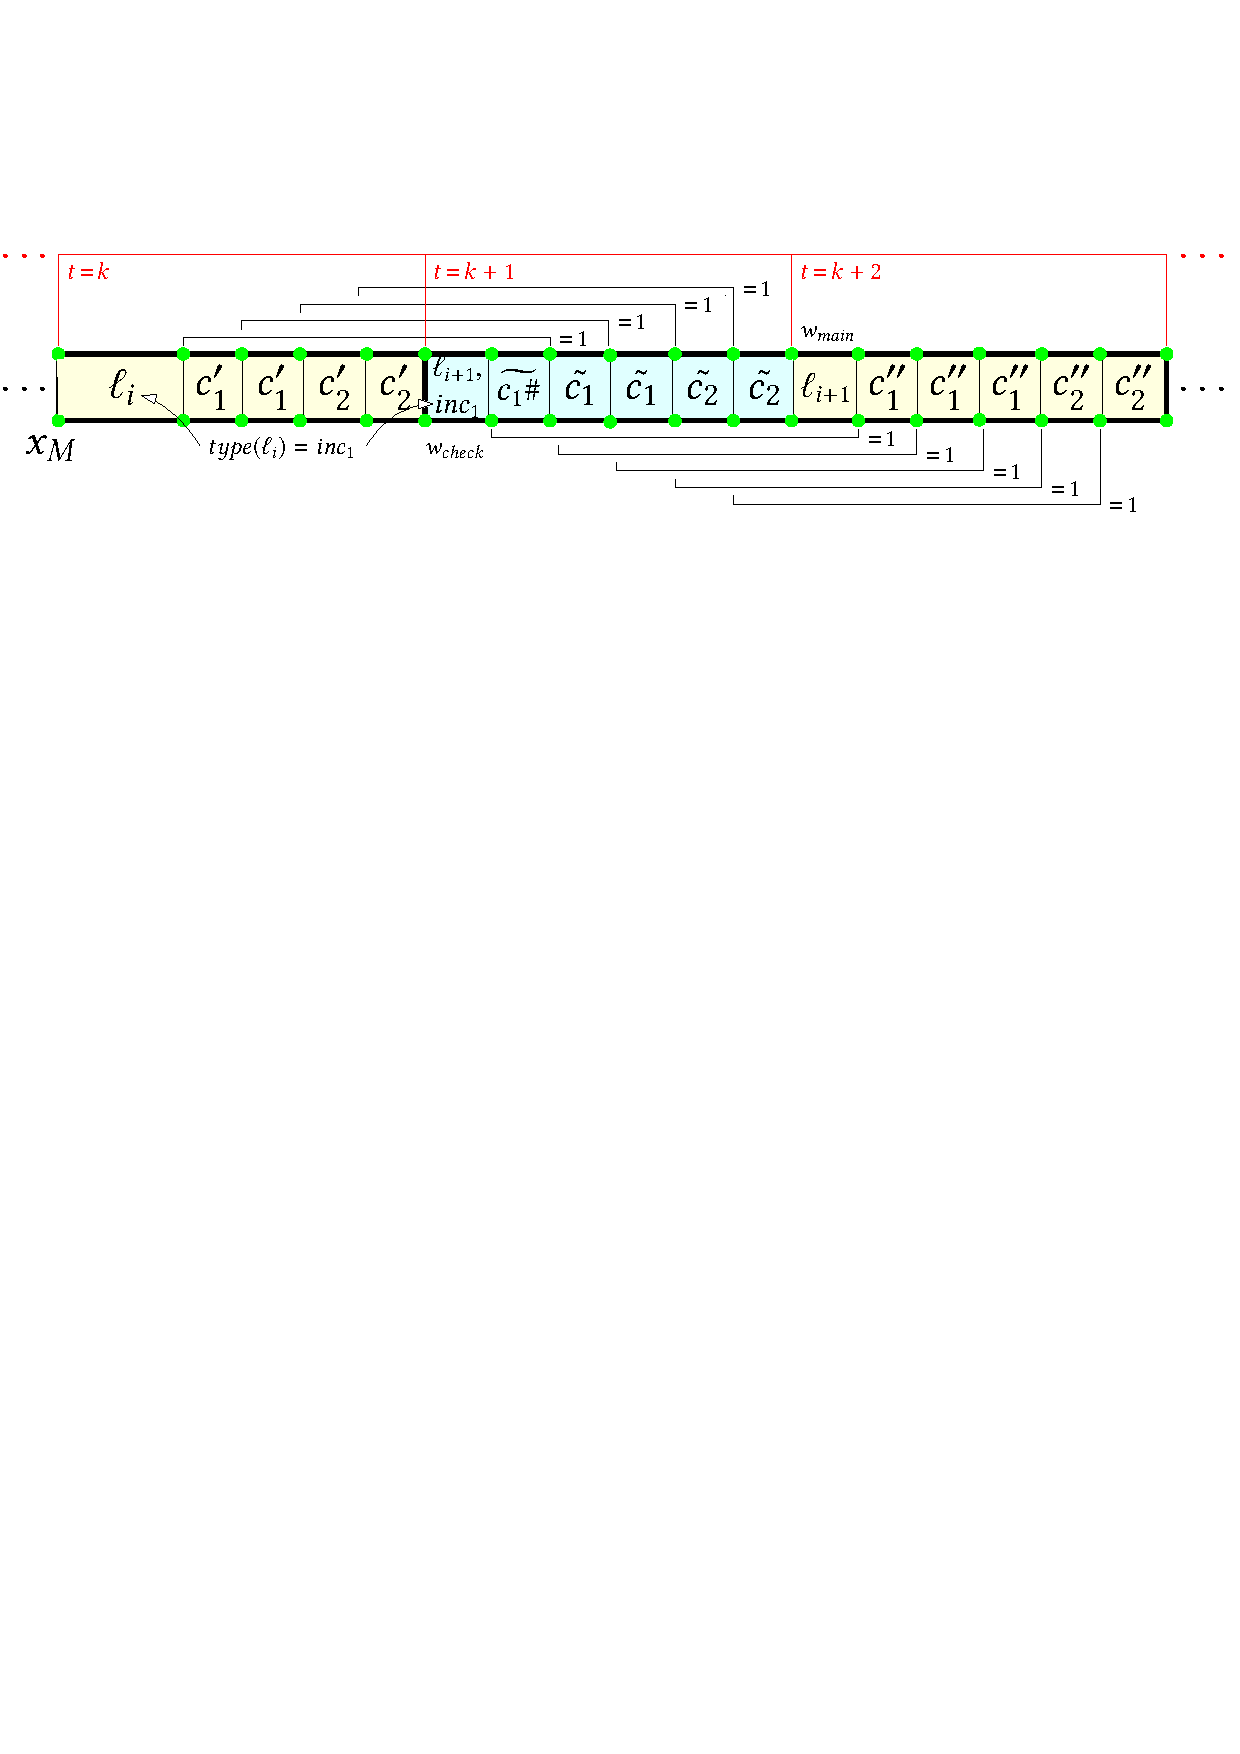
\includegraphics[width=\textwidth]{Chaps/Timelines/counters.pdf}
    \caption{
%  
A fragment of a computation code with a configuration code for 
an instruction $\ell_{i+1}$. Main-codes are highlighted in yellow and check-codes in cyan. Each square can also be seen as a token of a timeline for $x_M$ (tokens are decorated with their start time and their temporal constraints).
%%Encoding of a computation of $M$ as a timeline for $x_M$. 
%%We focus on the (simpler) case of increment instructions. 
%%A computation is given by the concatenation of main-codes (highlighted in yellow) and check-codes (in cyan). The first character (token) of a main-code is an instruction label, whereas the first character of a check-code is an instruction label, 
%%along with the type of the previous instruction (in the figure, $inc_1$ stands for an instruction incrementing $c_1$). 
%%The values of $c_1$ and $c_2$ are represented by the number of occurrences of tokens $c_1$ and $c_2$ respectively. 
%%Any check-code must have the same instruction label as the main-code \emph{following} it, and encode the same configuration.
%At every integer instant of time, we force some check- or main-code to begin. 
%
%%In order to ensure that a check-code $w_{check}$ represents the same value of $c_1$ (resp., $c_2$) as the following main-code $w_{main}$, we put into one-to-one correspondence an occurrence of $c_1$ (resp., $c_2$) in $w_{check}$ and one in $w_{main}$. To enforce this, the start time/point of each occurrence of $c_1$ (resp., $c_2$) in $w_{check}$ must be followed, \emph{after exactly 1 instant of time}, by the start time/point of the (corresponding) occurrence of $c_1$ (resp., $c_2$) in $w_{main}$ (as in the case of Metric Temporal Logic, singular intervals play a fundamental role here).
%To manage the increment of 1 unit of $c_1$, we force the same correspondence among \emph{unmarked} (i.e., without \#) occurrences of $c_1$ in $w_{check}$ and those of the \emph{preceding} main-code. There is a single token $c_1\#$ in $w_{check}$---that represents the unit added to $c_1$ by the instruction $\ell_i$---which does not correspond to any of the $c_1$'s of the preceding main-code. 
%%Let us observe that, since the time domain is \emph{dense}, in check-codes we can always add some more marked units $c_1\#$ in between the instruction label and the first unmarked occurrence of $c_1$.     
%    
In the figure, for $h\in\{1,2\}$, the symbols $c_h'$, $\tilde{c_h}$, $\widetilde{c_h\#}$, and $c_h''$, stand respectively for $(\ell_i ,c_h)$, $(\ell_{i+1},inc_1,c_h)$, $(\ell_{i+1},inc_1,(c_h,\#))$, and $(\ell_{i+1} ,c_h)$.
    }
    \label{fig:counters}
\end{figure}
A \emph{computation}-code is a %non-empty
sequence of configuration-codes $\pi= w_{\Checking}^{1}\cdot w_\main^{1}\cdots\allowbreak  w_{\Checking}^{n}\cdot w_\main^{n}$ such that, for all $1\leq j<n$, the following holds (we assume $\ell_i$ to be the instruction label associated with the configuration code $w_{\Checking}^{i}\cdot w_\main^{i}$):
%
\begin{itemize}
  \item $\ell_j\neq \ell_\halt$;
  \item if $\ell_j\in\Inc$ with $c(\ell_j)=c_h$, then $\ell_{j+1}=\Succ(\ell_j)$ and  $w_{\Checking}^{j+1}$ is associated with the operation
  $\inc_h$;
  \item if $\ell_j\in\Dec$ with $c(\ell_j)=c_h$, and the first symbol of $w_\main^{j}$ is $(\ell_j,\zero(\ell_j))$ (resp., $(\ell_j,\dec(\ell_j))$),
  then $\ell_{j+1}=\zero(\ell_j)$ (resp., $\ell_{j+1}=\dec(\ell_j)$) and  $w_{\Checking}^{j+1}$ is associated with the operation
  $\zero_h$ (resp., $\dec_h$).
\end{itemize}
%
The computation-code $\pi$ is \emph{well-formed} if, additionally, each configuration-code in $\pi$ is \emph{well-formed} and, for all $1\leq j<n$, the following holds  (we assume  $(\ell_i,n_1^{i},n_2^{i})$
to be the configuration encoded by $w_{\Checking}^{i}\cdot w_\main^{i}$):
%
\begin{itemize}
  \item if $\ell_j\in\Inc$, with $c(\ell_j)=c_h$,  then $n_h^{j+1}= n_h^{j}+1$ and $n_{3-h}^{j+1}= n_{3-h}^{j}$;
  \item if $\ell_j\in\Dec$, with $c(\ell_j)=c_h$, then $n_{3-h}^{j+1}= n_{3-h}^{j}$. Moreover, if  $w_{\Checking}^{j+1}$ is associated with %the operation
  $\dec_h$, then $n_h^{j+1}= n_h^{j}-1$.
\end{itemize}
%
Clearly, a well-formed computation code  $\pi$ encodes a computation of the Minsky 2-counter machine. 

A computation-code $\pi$ is \emph{initial} if it starts with the  prefix $(\ell_\init,\zero_1)\cdot  \ell_\init$, and it is \emph{halting} if it leads to a configuration-code associated with the halting label $\ell_\halt$. The counter machine $M$ halts if and only if there is an initial and halting well-formed computation-code.

\paragraph*{Definition of $x_M$ and $R_M$.}
Let us show now how to reduce the problem of checking the existence of an initial and halting well-formed computation-code to a TP problem for the state variable $x_M$. 

The idea is to define a timeline where the sequence of values of its tokens is a well-formed computation-code. The durations of tokens are suitably exploited to guarantee well-formedness of computation-codes. We refer the reader again to Figure~\ref{fig:counters} for an intuition. 
Each symbol of the computation-code is associated with a token having a positive duration. The overall duration of the sequence of tokens corresponding to a check-code or a main-code amounts exactly to one time unit. To allow for the encoding of 
%possibly unbounded 
arbitrarily large values of counters in one time unit, the duration of such tokens is not fixed (taking advantage of the dense temporal domain). In two adjacent check/main-codes, the time elapsed between the start times of corresponding elements in the representation of the value of a counter (see elements in Figure~\ref{fig:counters} connected by horizontal lines) amounts exactly to one time unit. Such a constraint allows us to compare the values of counters in adjacent codes, either checking for equality, or simulating (by using marked symbols) increment and decrement operations. Note that there is a single \emph{marked} token $c_1$ in the check-code---that represents the unit added to $c_1$ by the instruction $\ell_i$---which does not correspond to any of the $c_1$'s of the preceding main-code.

We now formally define a state variable $x_M$ and a set $R_M$ of synchronization rules for $x_M$ such that the untimed part of any timeline (i.e., neglecting tokens' durations)
for $x_M$ satisfying the rules in $R_M$ is (represents) an initial and halting well-formed computation-code. Thus, $M$ halts if and only if there exists a timeline for $x_M$ satisfying the rules in $R_M$.

As for $x_M$, we let $x_M= (V,T,D)$ where, for each $v\in V$, 
%we have 
$D(v)=\mathopen]0,1\mathclose]$. This sets the \emph{strict time monotonicity} constraint, namely, the duration of a token along a timeline is always greater than zero and less than or equal to 1. 

The value transition function $T$ of $x_M$ ensures the following requirement.
\begin{claim}\label{ref:claim}
The untimed part of any timeline for $x_M$ whose first token has value $(\ell_\init,\zero_1)$
 is a prefix of some initial computation-code. Moreover, $(\ell_\init,\zero_1)\notin T(v)$ for all $v\in V$.
\end{claim}
It is a straightforward task to define $T$ in  such a way that the previous requirement is fulfilled (for details, see Appendix~\ref{sec:undecidabilityTrans}).
 
Finally, the synchronization rules in $R_M$ ensure the following requirements.
%
 \begin{itemize}
%   \item \emph{Strict time monotonicity:}  the duration of a token along a timeline is always greater
%   than zero and less or equal to 1. This is expressed by the following rules: for all $v\in V$, 
%   %
%   $
%   o[x_M=v] \rightarrow o\leq^{\start,\End}_{(0,1]} o 
%   $.
%   %
   \item \emph{Initialization:} every timeline starts with two tokens, the first one having value
   $(\ell_\init,\zero_1)$, and the second having value $\ell_\init$. By Claim~\ref{ref:claim} and the fact that no instruction
   of $M$ leads to $\ell_\init$, it suffices to require that a timeline has a token with value $(\ell_\init,\zero_1)$ and a token with value
   $\ell_\init$.
   This is ensured by the following two trigger-less rules:
   %
   \[
   \true \rightarrow \exists \, o[x_M=(\ell_\init,\zero_1)].\, \true
   \] and \[
   \true \rightarrow \exists \, o[x_M= \ell_\init].\, \true
   .\]
   %
   \item \emph{Halting:} every timeline leads to a configuration-code associated with the halting label. By the rules for initialization and Claim~\ref{ref:claim}, it suffices to require that a timeline has a token with value $\ell_\halt$. This is ensured by the following trigger-less rule:
   %
   \[
   \true \rightarrow \exists \, o[x_M=\ell_\halt].\, \true
   .\]
   %
    %
   \item \emph{1-Time distance between consecutive control values:} a \emph{control $V$-value} corresponds to the first symbol of a $\main$-code or a $\Checking$-code, i.e., it is an element in $V\setminus (V_{c_1}\cup V_{c_2})$. We require  that the difference of the start times of two consecutive tokens along a timeline having a control $V$-value is exactly $1$. Formally, 
%      in other terms, 
    for each pair $tk$ and $tk'$ of tokens along a timeline such that $tk$ and $tk'$ have a control $V$-value, $tk$ precedes $tk'$, and there is no token between $tk$ and $tk'$ having a control $V$-value, it holds that $\startTime(tk')-\startTime(tk)=1$ (we write this with a little abuse of notation). By Claim~\ref{ref:claim}, strict time monotonicity, and the halting requirement, it suffices to ensure that each token $tk$ having a control $V$-value distinct from $\ell_\halt$ is eventually followed by a token $tk'$ such that $tk'$ has a control $V$-value and $\startTime(tk')-\startTime(tk)=1$. To this aim, for each  $v\in V_\Con\setminus \{\ell_\halt\}$, being $V_\Con$ the set of control $V$-values,  we write the following trigger rule:
    %
   \[
   o[x_M=v] \rightarrow \displaystyle{\bigvee_{u\in V_\Con}} \exists\, o'[x_M= u].\, o\leq^{\start,\start}_{[1,1]} o'. 
   %\\ \text{for each } v\in V_\Con\setminus \{\ell_\halt\}.
   \]
   
   \item \emph{Well-formedness of configuration-codes:} we need to guarantee that for each configuration-code $w_\Checking\cdot w_\main$ occurring along a timeline and 
%for 
    each counter $c_h$, the value of $c_h$ along the $\main$-code $w_\main$ and the $\Checking$-code $w_\Checking$ coincide.
    By Claim~\ref{ref:claim}, strict time monotonicity, initialization, and 1-Time distance between consecutive control values,  it suffices to ensure that $(i)$~each token $tk$  with
    a $V_{c_h}$-value in $V_\Checking$ is eventually followed by a token $tk'$ with a $V_{c_h}$-value such that  $\startTime(tk')-\startTime(tk)=1$, and vice versa $(ii)$~each token $tk$  with
    a $V_{c_h}$-value in $V_\main$ is eventually preceded by a token $tk'$ with a $V_{c_h}$-value such that  $\startTime(tk)-\startTime(tk')=1$. As for the former requirement, for each   $v\in V_{c_h}\cap V_\Checking$, we write the rule:
    %
   \[
   o[x_M=v] \rightarrow \displaystyle{\bigvee_{u\in V_{c_h}}} \exists\, o'[x_M= u].\, o\leq^{\start,\start}_{[1,1]} o'.
   %\\ \text{for each }  v\in V_{c_h}\cap V_\Checking.
   \]
   
   For the latter, for each   $v\in V_{c_h}\cap V_\main$, we have the rule:
       %
   \[
   o[x_M=v] \rightarrow \displaystyle{\bigvee_{u\in V_{c_h}}} \exists\, o'[x_M= u].\, o'\leq^{\start,\start}_{[1,1]} o.
   %\\ \text{for each } v\in V_{c_h}\cap V_\main.
   \]
   
   \item \emph{Increment and decrement:} we need to guarantee that the increment and decrement instructions are correctly simulated.
    By Claim~\ref{ref:claim} and the previously defined synchronization rules, we can assume that the untimed part $\pi$ of a timeline is an initial and halting
    computation-code such that all  configuration-codes occurring in $\pi$ are well-formed.

    Let $w_\main \cdot w_\Checking$ be a subword occurring in $\pi$ such that
    $w_\main$ (resp., $w_\Checking$) is a $\main$-code (resp., $\Checking$-code). Let $\ell_\main$ (resp., $\ell_\Checking$) be the instruction label
    associated with $w_\main$ (resp., $w_\Checking$) and for $i=1,2$, let $n_i^{\main}$ (resp., $n_i^{\Checking}$) be the value of counter $c_i$ encoded by
     $w_\main$ (resp., $w_\Checking$). Let $c_h=c(\ell_\main)$. By construction $\ell_\main\neq \ell_\halt$, end either $\ell_\main\in\Inc$   and
     $\ell_\Checking =\Succ(\ell_\main)$, or $\ell_\main\in \Dec$  and $\ell_\Checking\in \{\zero(\ell_\main),\dec(\ell_\main)\}$. Moreover, if $\ell_\main\in \Dec$
     and $\ell_\Checking = \zero(\ell_\main)$, then $n_h^{\Checking}= n_h^{\main}=0$.
     Thus, it remains to ensure the following two requirements:
     \begin{itemize}
       \item[(*)] if $\ell_\main\in\Inc$, then $n_h^{\Checking}= n_h^{\main}+1$ and $n_{3-h}^{\Checking}= n_{3-h}^{\main}$;
       \item[(**)] if $\ell_\main\in\Dec$, then $n_{3-h}^{\Checking}= n_{3-h}^{\main}$, and whenever
       $\ell_\Checking = \dec(\ell_\main)$, then $n_h^{\Checking}= n_h^{\main}-1$.
     \end{itemize}

First we observe that, if $\ell_\main\in\Inc$, our encoding ensures that all $V_{c_{3-h}}$-values in $w_\main$ and in $w_\Checking$ are unmarked,
all $V_{c_{h}}$-values in  $w_\main$ are unmarked, and there is exactly one marked $V_{c_{h}}$-value  in  $w_\Checking$.
If instead $\ell_\main\in\Dec$, our encoding ensures that all $V_{c_{3-h}}$-values in $w_\main$ and in $w_\Checking$ are unmarked,
all $V_{c_{h}}$-values in  $w_\Checking$ are unmarked, and in case $\ell_\Checking= \dec(\ell_\main)$, then there is exactly one marked $V_{c_{h}}$-value  in  $w_\main$.
Thus, by strict time monotonicity and 1-Time distance between consecutive control values, it follows that requirements~(*) and~(**) are captured by the following
rules, where $U_{c_i}$ denotes the set of \emph{unmarked} $V_{c_i}$-values, for $i=1,2$, and $V_\init$ (resp., $V_\halt$) is the set of $V$-values associated with the label $\ell_\init$ (resp., $\ell_\halt$). For each   $v\in (U_{c_i}\cap V_\main)\setminus V_\halt$, we have the rule:
 %
   \[
   o[x_M=v] \rightarrow \displaystyle{\bigvee_{u\in U_{c_i}}} \exists\, o'[x_M= u].\, o\leq^{\start,\start}_{[1,1]} o'. 
   %\\ \text{for each }  v\in (U_{c_i}\cap V_\main)\setminus V_\halt
   \]
   
   For each $v\in (U_{c_i}\cap V_\Checking)\setminus V_\init$, we have the rule:
   \[
   o[x_M=v] \rightarrow \displaystyle{\bigvee_{u\in U_{c_i}}} \exists\, o'[x_M= u].\, o'\leq^{\start,\start}_{[1,1]} o .
   %\\ \text{for each } v\in (U_{c_i}\cap V_\Checking)\setminus V_\init \qedhere
   \]
 \end{itemize}
This concludes the proof of the theorem.
\end{proof}

It is worth observing that all the above trigger rules are \emph{simple}, hence \emph{undecidability of the TP problem holds also under the restriction to simple trigger rules}.

In order to ensure the well-formedness of configuration-codes and the increment/decrement requirements, a one-to-one correspondence between (suitable) pairs of tokens in main- and check-codes is enforced thanks to the above trigger rules. Whereas most of such rules are (already) satisfied under the future semantics (as the extra conjoined atoms added by Definition~\ref{def:futurerules} would be \lq\lq subsumed\rq\rq\ by already-existing ones), some rules are not (the second ones of the well-formedness and increment/decrement requirements are unsatisfiable under the future semantics). 
As a result, intuitively, having only rules under the future semantics,
we can only force the presence, for every token with value $c_h$ (for $h=1,2$), of another token with value $c_h$ starting exactly one time instant later, in the following main-/check-code. However, we cannot prevent extra \lq\lq spurious\rq\rq\  tokens to appear moving from a code to the following one.
This is the reason why, with only rules under the future semantics, we lose the ability of encoding computations of (exact) Minsky machines. Only \emph{gainy counter machines}~\cite{DemriL09}---a variant of Minsky machines whose counters may \lq\lq erroneously\rq\rq\ increase---can be captured, thus proving, as a consequence, 
\emph{non-primitive recursive-hardness} of the future TP problem (the halting problem for gainy counter machines is known to be non-primitive recursive~\cite{DemriL09}). 

\begin{theorem}\label{theorem:NPRHardness}
The future TP problem, even with \emph{one state variable}, is non-primitive recursive-hard also under one of the following two assumptions: \emph{either} $(1)$ the trigger rules are simple,
\emph{or} $(2)$ the intervals are in $\Intv_{(0,\infty)}$%
\footnote{We refer to intervals in rules' atoms and in the constraint functions of state variables.}.
\end{theorem}

Since this result is just an adaptation of the previous one (apart from some technicalities), we report its proof in Appendix~\ref{sec:NPRHardness}. 
%As we show there, 
%non-primitive recursive-hardness holds also with just one state variable, and again with the restriction to simple trigger rules.

In the next section, we will show that future TP with simple trigger rules is indeed decidable in non-primitive recursive time. 